\section{Introduction}

	Humans, while looking at an object, at the first glance perceive the gross shape and then eventually look into more details as needed \cite{LeeLee1998}. This process of simplification of the shape, by ignoring the small and irrelevant details is widely used in geometric computations and is referred to as ``Defeaturing''.  It is the process of suppressing some features based on certain predefined objectives or criteria.
	
		Many existing simplification methods recognize small, irrelevant features on a mesh or a solid body first, then remove them to get the simplified (called ``defeatured'') model. Instead, if a Feature-based CAD model is used as an input, then it has the advantage of the availability of ready features, so that the suppression and healing becomes relatively straightforward and robust. In such a feature-based defeaturing method, the primary challenge is the identification of the suppressible features. In the past, the suppressibility used to be based on some insufficient criteria, like using full feature parameters, selecting all the negative features, etc. 
Defeaturing is primarily used in CAE analysis where such simplified models lower the complexity of the finite element mesh and thus reduce the analysis time. It is also used in shape matching \& retrieval, fast visualization, hiding proprietary details, transmission across network, finding gross shape, etc. This paper focuses on using defeaturing for finding the gross shape needed in the computation of a medial form, called ``Midsurface'' \cite{Ramanathan2004}. Gross shape is the principal shape that “represents” the given shape but with far lesser features. Gross-ness depends on the size criteria, say, 5\% of the total volume/area. Features having sizes below this are the candidates for suppression. With lesser irrelevant details on the input model, the generated midsurface becomes more representative of the original part and the computation becomes robust (small deviations/features in the input do not affect the output in appreciable manner).

Tab. \ref{tab_defeatmids}  shows the result of an experiment to see whether the defeaturing helps in the quality of the midsurface. The first row shows the original model, its midsurface (with a problem shown in red circle) and the same problem shown in a magnified manner. The second row shows the defeatured model, its midsurface and mentions quality of the midsurface output.  The third row shows that even though the defeaturing has positive effect on the midsurface output, it should be done judiciously to retain enough features in the midsurface as well.

\begin{center}
\begin{tabular}[h]{@{} p{0.17\linewidth}  p{0.25\linewidth} p{0.25\linewidth} p{0.25\linewidth}@{}} \toprule
\textbf{Part \& actions} & \textbf{Model} & \textbf{Midsurface} & \textbf{Problems} \\ \midrule

Original model & 
\adjustbox{valign=t}{
 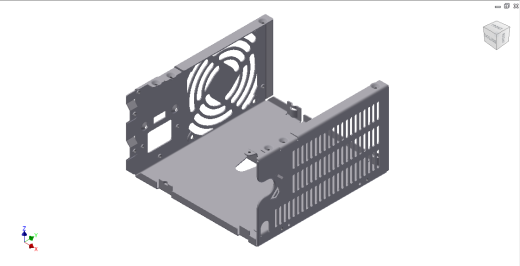
\includegraphics[width=\linewidth]{../Common/images/defeatmids_origpart} 
} &

\adjustbox{valign=t}{
 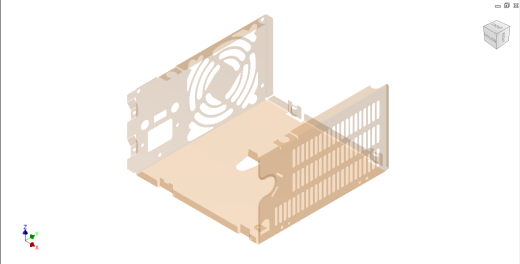
\includegraphics[width=\linewidth]{../Common/images/defeatmids_origmids} 
} &

Gaps and missing surfaces
\adjustbox{valign=t}{
 
\includegraphics[width=0.4\linewidth, angle=90]{../Common/images/defeatmids_origprobs} 
 } 

 \\

Manual defeaturing of the small irrelevant features. & 
\adjustbox{valign=t}{
 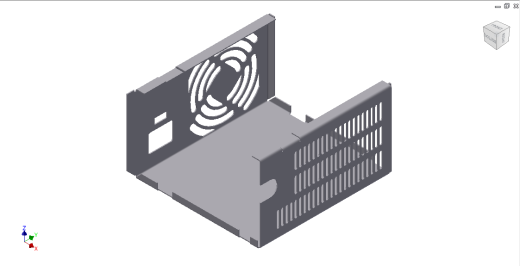
\includegraphics[width=\linewidth]{../Common/images/defeatmids_finpart} 
} &

\adjustbox{valign=t}{
 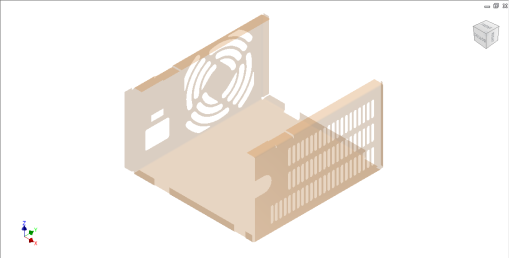
\includegraphics[width=\linewidth]{../Common/images/defeatmids_finmids} 
} &

No major errors in the midsurface such as gaps, missing surfaces, etc. Such output is desirable. \\

All negative features suppressed. & 
\adjustbox{valign=t}{
 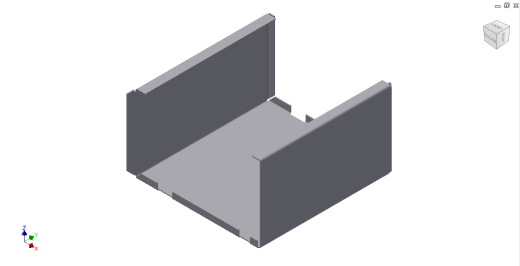
\includegraphics[width=\linewidth]{../Common/images/defeatmids_negpart} 
} &

\adjustbox{valign=t}{
 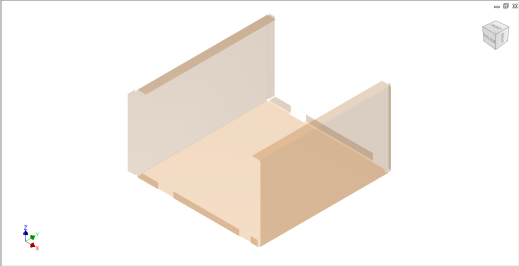
\includegraphics[width=\linewidth]{../Common/images/defeatmids_negmids} 
} &

Midsurface does not have errors, such as gaps or missing surfaces but it is missing some important features.\\

\bottomrule
\end{tabular}
\captionof{table}{Effect of Defeaturing on the Midsurface Generation} \label{tab_defeatmids}
\end{center}

Defeaturing has largely been a manual and tedious process. Small and irrelevant features are first recognized in the mesh/solid body based on the heuristic rules and removed \cite{BelazizBourasBrun2000}. Finally the model is healed to form a closed watertight shape. Users view this task as too extensive and resort to recreate the necessary geometry than to simplify the existing one \cite{Halpern1997}. 

Objective of this work is to develop a computational method to automatically find simplified geometry of a sheet metal part model which can be used for further computations such as the generation of the midsurface. The method works in two phases. In the first, the objective is to identify and classify sheet metal features into suppressible and non-suppressible features, based on type and size criteria. Such classification has been presented in the form of taxonomy. In the second phase, a generic method based on geometric reasoning is proposed to identify the suppressible features. 

	
\section{Related Work}	
Research in simplification of geometry has been going on for decades.  And\'ujar \cite{Andujar99} surveyed various geometric simplification techniques with input as mesh models, and for applications such as visualization, interface detection, visibility analysis, and transmission of models. He stated that the geometric fidelity and entity reductions are opposite goals, and thus, choice of a validation criterion dictates the quality of the output as well as appropriateness to the end application. 
	
	Kim et al. \cite{Kim2005} demonstrated the use of operators like wrap-around and smoothing to fill up small holes, concave shapes and protrusions. The approaches presented in that work appear simplistic and would not get scaled for the complex parts.
	
	Defeaturing is one of the most popular techniques of simplification for CAE analysis. Thakur et al. \cite{Thakur2009}surveyed and classified various techniques used till then, into four categories such as surface-based, volume-based, feature-based, and dimension-reduction.  Most methods were based on mesh and solid as the input, with very few based on the feature-based CAD model. The work presented in the current paper is based on defeaturing with feature-based CAD model.

Feature-based design represents a CAD model in terms of a feature tree where each tree-node is termed as a {\em feature}.  Features not only present modeling in the application-specific-vocabulary to the designers, but also provide parametric editing capabilities. The designers can update the models based on critical driving parameters. They can also suppress certain features and update the model to regenerate the shape. Such capabilities are (and can be) immensely leveraged in the defeaturing algorithms. Another advantage of using feature-based design is in the regeneration of the original model. As during defeaturing, features are only suppressed and not deleted. So, if there is a need to regenerate the original model, the suppressed features can simply be unsuppressed.

Nowadays, many CAD modelers are based on the feature-based design paradigm and provide access to the feature tree. Feature-based defeaturing operations have better applicability than mesh or solid based simplification methods for product design and engineering applications  \cite{Kang2013}. They also provide ready APIs (Application Programming Interfaces) to exclude/suppress certain features while computing the final shape. Feature based defeaturing methods are reviewed in the following section.

\subsection{Feature-based Defeaturing}

Dabke \cite{Dabke1994} through the concept of ‘global idealization’, was one of the first researchers to leverage the feature information for defeaturing. This method was based on the expert system with heuristic rules derived from the analyst's experience. The proposed approach appears to be rudimentary in the usage of features.

Lee \cite{Lee2005, SangHunLee2005, Lee2009} elaborated a method to reorder the design features in the history tree and then to re-execute the history of the reordered features up to the given level of simplification. Since Brep (Boundary representation) re-evaluation is computationally intensive, he used the cellular model for increasing the performance. One of the major limitations of this approach is that once the model is converted to cellular, its feature update capability would cease to exist, making it difficult for bidirectional change propagation.
	 
 Smit \cite{Smit2009} surveyed various approaches for CAD-CAE integrations and concluded that since features carry domain-specific information, they can bring context-relevant defeaturing. With this ease, there also comes one complication. Many features are built using entities from the existing features, creating dependencies called "parent-child" relationships. Suppressing a parent feature suppresses the child features too. Deciding the eligibility of suppression of the feature should thus include child features too. Otherwise, one has to build/adopt the part in such a way that the dependencies are removed or rerouted \cite{AmesRiveraWebbHensinger1997}.

Feature trees may be different for similar final shapes. So, defeaturing based on the feature tree can yield different results. To achieve consistent defeaturing results independent of the modeling history, some attempts use just the final solid (Brep) model, and then recognize the features \cite{Woo2009} to be removed directly from that final model. Even if there are a few limitations on the usage of the feature tree as stated above, having ready feature information is far convenient for defeaturing than doing feature recognition first and then suppressing the qualified ones. 

Woo \cite{Woo2009} proposed a new method which has subtractive features recognized directly from the final solid, thus eliminating the problem of looking at the history tree. It lacked coverage in terms of variety of features being recognized and thus, was limited to simple shapes

	Hamdi et al. \cite{Hamdi2012a} also surveyed simplification techniques and classified them based on the input format, features simplified, defeaturing criterion, advantages, limitations and application domain. Most of the methods were Brep-based and suppressed features like holes, chamfers, fillets, protrusions, depressions, passages, concave regions, etc. They used geometric reasoning (size criterion) as well as application-specific rules (boundary conditions and proximity with loading zone) for identification of the suppressible features.  
	

Russ \cite{Russ2012} mentioned that the determination of the non-critical (suppressible) features relies on different attributes of not only the features themselves, but also of the entire part model and analysis. Some of these attributes include the feature type, feature dimensions, proximity of features to the boundary conditions, analysis type, and part dimensions. He used full feature parameters for deciding the eligibility of the suppression. 

The selection criteria for suppressing the features, apart from being application-specific, are based on the targeted accuracy, cost or preparation time, etc \cite{Danglade2013}. Looking at the variety of inputs, types of analysis and application domains, it is difficult to quantify and generalize. So, each domain typically presents its own feature taxonomy with regards to defeaturing to decide the eligibility for suppression.
	
	Danglade \cite{Danglade2013} used machine-learning techniques to capitalize the knowledge and experience; where the analysts have to provide the decision making for the defeaturing step. After a large number of learning trials, the system itself suggests relative necessity of the features and their impact on the accuracy of the results.

Joshi and Dutta \cite{Joshi2003}  recognized the sheet metal features on free-form surfaces and then suppressed them for simplification. Their work appears to be limited to only holes, fillets and bosses.

	Kang et al. \cite{Kang2013} customized the defeaturing criteria for shipyard requirements where, apart from geometric reasoning criteria such as volume, they included application-specific rules for ports and outer boundary. 
	
	Commercial packages like ACIS\textsuperscript{\textregistered}, Autodesk Fusion\textsuperscript{\textregistered}, Altair's Hypermesh\textsuperscript{\textregistered} also to provide similar defeaturing capabilities mainly for CAE analysis.
	
Some important conclusions based on the literature survey of feature-based defeaturing are:
\begin{itemize}
[noitemsep,topsep=2pt,parsep=2pt,partopsep=2pt,label=\textbullet]
\item Identification of the suppressible features, just by their types, cannot be used blindly across all domains. For example, a rib-like feature may not be relevant in the metal flow analysis but may be relevant in the heat transfer analysis. So, there is a need for domain-specific identification rules, such as rules for sheet metal domain, shipbuilding, etc.
\item  Geometric reasoning can be used for size-based identification of the suppressible features. Based on the engineering judgment, a size threshold may be decided, below which features can be suppressed. Here, the calculation of the feature size becomes critical as it decides the eligibility for suppression. Full feature dimensions are used by some of the past approaches \cite{Kang2013} \cite{Russ2012} giving wrong results, as the feature is not fully present in the final shape. 
\end{itemize}
The work presented in this paper focuses on feature-based defeaturing specific to sheet metal parts. Sheet metal parts are prevalent in industries, such as automotive, aerospace, process, electronics, etc. Clear definition and classification of sheet metal features is a prerequisite in deciding the defeaturing rules. Some of the available classifications for sheet metal features are reviewed in the following section.

	
\subsection{Sheet Metal Features}

Liu et al. \cite{Liu2004} stated that a sheet metal CAD part model is made up of base features (Wall/Face feature) upon which several child/secondary features (Cutouts, etc.) are positioned. Then, the tertiary and connector features are added to complete the desired shape. They classified sheet metal features into Primitives features which are independent features, Add-ons which are on the Primitives, Connectors which connect the features and Composites which are made up of the earlier-defined types.

Sunil \cite{Sunil2008} classified sheet metal features into face-based features which lie on the face (holes, dimple, and beads), edge-based features (flange, ridge) which lie on the periphery of the part, while transitive features (bend) lie between the faces.

Survey suggests that for a well-connected midsurface, primitive and connecting/transitive features are critical and they need to be retained, whereas secondary features can be suppressed by comparing their size relative to the given threshold. 

This paper proposes a novel method to address the stated issues. Section 3 presents details of the method using two phases and algorithms (Subsection \ref{ph1} and \ref{ph2}) whereas in Section \ref{results} we present the results with case studies.
